\section{Bazy danych i ADO.NET}

\subsection{Interfejsy komunikacji z bazami danych}

Pisząc aplikację, której zadaniem jest gromadzenie i przetwarzanie informacji, programista
często staje przed wyborem sposobu gromadzenia danych. Współcześnie najczęściej wykorzystuje się
do tego serwery baz danych, bowiem gwarantują one, m.in bezpieczeństwo, integralność i nienaruszalność danych.

Z punktu widzenia programisty, serwer baz danych jest zwykłym programem, który swoje usługi dostępu do danych
oferuje wielu klientom. Schemat takiej komunikacji jest identyczny jak znany nam już z poprzednich rozdziałów
schemat wymiany danych między serwerem, a klientem sieciowym: jakiś protokół {\bf fizyczny} pełni rolę
nośnika informacji, zaś jakiś protokół {\bf logiczny} określa postać wymienianych komunikatów.

Interfejsy programowania baz danych zwalniają programistę z konieczności czuwania nad szczegółami
komunikacji, pozwalają zaś skupić się na wymianie danych między klientem a serwerem. Jak zobaczymy
w kolejnych podrozdziałach, istnieją trzy podstawowe operacje udostępniane przez interfejs
programowania baz danych, których programista musi użyć do komunikacji z serwerem:
\begin{enumerate}
\item Otwarcie połączenia z wybranym serwerem baz danych
\item Wykonanie operacji na otwartym połączeniu
\item Zamknięcie połączenia do bazy danych
\end{enumerate}

Możliwości oferowane przez poszczególne serwery baz danych różnią się od siebie. Mogłoby się więc wydawać, że
interfejs programowania serwera MySQL, Microsoft SQL Server, czy Oracle muszą się od siebie różnić. Na szczęście
nie jest aż tak źle, opracowano bowiem takie interfejsy, które są oderwane od
szczegółów implementacji konkretnego serwera i (przynajmniej teoretycznie) pozwalają oprogramować komunikację z 
każdym dostępnym serwerem baz danych w dokładnie taki sam sposób.

\subsubsection{ODBC}

{\bf Open DataBase Connectivity } jest interfejsem umożliwiającym dostęp do danych składowanych w 
dowolnym systemie zarządzania bazami danych ({\bf DataBase Maganement System}, 
DBMS\footnote{DBMSami są na przykład serwery baz danych.}). ODBC jest zbudowany w oparciu o specyfikacje
X/Open i ISO/IEC. 

W systemie Windows za komunikację z systemami zarządzania baz danych odpowiada biblioteka
{\bf odbc32.dll}. Zaimplementowano wiele sterowników ODBC dla różnych DBMSów. Jeśli na rynku
pojawia się nowy system bazodanowy, to jest niemal pewne, że będzie on potrafił 
komunikować się za pomocą ODBC. System Windows potrafi komuikować się za pomocą ODBC m.in. z MS SQL Severem,
Oracle, Visual Fox Pro, czy bazami MS Access. Producenci nowych rozwiązań bazodanowych najczęściej
sami dostarczają odpowiednie sterowniki, tak jest na przykład w przypadku serwera MySQL.

\subsubsection{OLE DB}

OLE DB jest rozwinięciem idei ODBC. 
W teorii umożliwia dostęp do dowolnych danych, nie tylko relacyjnym DBMSów. 

Idea OLE DB polega na współistnieniu trzech rodzajów obiektów. Są to:
\begin{itemize}
\item dostawcy danych ({\em data providers}), którzy przechowują i udostępniają dane
\item konsumenci danych ({\em data consumers}, którzy mogą korzystać z danych
\item składniki usługowe ({\em service components}), które przetwarzają dane
\end{itemize}

Obiekty z każdej z tych grup muszą po prostu udostępniać pewien ściśle określony (przez standard OLE DB)
zbiór funkcji. Teoretycznie można sobie wyobrazić na przykład taki scenariusz, w którym dostawca danych
przechowuje dane w pliku tekstowym, składnik usługowy te dane sortuje, zaś konsument pobiera wynik.

\subsubsection{ADO i ADO.NET}

Tak naprawdę programista piszący aplikacje klienckie raczej nigdy nie będzie zmuszony do pisania
własnych obiektów - dostawców danych, ani własnych usług OLE DB. Obie te funkcje
spełniane są przez systemy zarządzania bazami danych i istotne są z punktu widzenia projektantów
tych systemów. Programista aplikacji klienckiej jest za to zainteresowany interfejsem programowania
przeznaczonym do konsumowania danych udostępnianych przez systemy bazodanowe. Najpopularniejszym
interfejsem programowania konsumentów danych, dodatkowo opakowującym interfejs OLE DB, jest ADO.

Interfejs ADO ({\bf ActiveX Data Objects}) został zaprojektowany jako interfejs obiektowy,
udostępniany w modelu COM. Zdobył dużą populaność wśród programistów, ponieważ szybko powstały
komponenty ADO dla popularnych systemów RAD ({\bf Visual Basic}, {\bf Delphi}, języki skryptowe).
Siłą ADO od początku była jego prostota i jednorodność - ADO umożliwia pisanie aplikacji
w dużym stopniu niezależnych od sposobu składowania danych.

ADO.NET jest kolejnym krokiem w stronę uproszczenia interfejsu klienta OLE DB, dostępnego
dla programistów aplikacji na platformie .NET. Dzięki ADO.NET dostęp do baz danych wygląda niemal
identycznie nie tylko w różnych językach platformy .NET, ale jest niezależny od dostawcy danych.
Oznacza to, że praktycznie nie powinno mieć większego znaczenia czy składowiskiem danych aplikacji
jest MySQL, MS SQL Server czy Oracle, bowiem aplikacja komunikuje się z nimi wszystkimi w prawie 
identyczny sposób.

Dla połączeń OLEDB, interfejs ADO.NET udostępnia szereg klas, których nazwy rozpoczynają się od {\bf OleDb...},
na przykład {\bf OleDbConnection}. Specjalnie dla MS SQL Servera przygotowano specjalizowany
zestaw klas przeznaczonych wyłącznie dla MS SQL Servera, których funkcjonalność jest
identyczna, tyle że ich nazwy rozpoczynają się od {\bf Sql...}. Inni dostawcy systemów baz danych
podjęli tę konwencję, przygotowując specjalizowane klasy dla komunikacji z serwerem Oracle czy MySQL.

Zaletą specjalizowanych klas jest ich szybkość. Na przykład dzięki użyciu klas {\bf Sql...} aplikacja
wymienia dane z serwerem MS SQL około 2 razy szybciej niż za pomocą klas {\bf OleDb...}. 

Ich wada polega
zaś na tym, że obsługują tylko jeden typ dostawcy danych, w przeciwieństwie do klas {\bf OleDb...}, które
są ogólne i jedyna różnica w dostępie do danych z różnych serwerów wynika z konieczności
nieco innego zainicjowania połączenia do bazy danych.

\subsection{Manualne zakładanie bazy danych}

Sposoby wymiany danych między serwerem bazy danych a aplikacją omówimy na przykładzie
serwera bazodanowego Microsoft SQL Server. Wymiana danych z innymi serwerami baz danych
wygląda identycznie od strony interfejsu programowego. Różnice mogą pojawiać się tylko
wtedy, kiedy serwer bazodanowy, z którym komunikuje się aplikacja, nie obsługuje
pewnych mechanizmów, których spodziewa się aplikacja. 

Przykład rozpoczniemy od założenia bazy danych. Większość serwerów baz danych wspomaga operacje administracji 
specjalnymi narzędziami z wygodnym interfejsem użytkownika\footnote{W przypadku serwera MS SQL Server, okienkowym
narzędziem administracyjnym może być nawet Microsoft Access}, jednak prawie zawsze dają możliwość korzystania
bezpośrednio z poleceń języka SQL. 

Skorzystamy więc z tej możliwości, aby utworzyć prostą bazę danych na serwerze MS SQL Server. Do każdej wersji
serwera SQL Server (dotyczy to nawet wersji "Desktop", czyli MSDE) dołączone jest narzędzie o nazwie {\bf osql}, które
pozwala na wydawanie poleceń SQL serwerowi.

Zacznijmy od połączenia się ze wskazanym serwerem (nazwa {\bf (local)} oznacza serwer lokalny) jako wskazany
użytkownik. MS SQL Server może podczas pracy używać własnych mechanizmów uwierzytelniania, niezależnych
od uwierzytelniania w systemie. W takim scenariuszu administrator serwera nazywa się {\bf sa} i on tworzy
kolejnych użytkowników i nadaje im uprawnienia do korzystania z poszczególnych baz danych. 

\begin{scriptsize}
\begin{verbatim}
C:\MSSQL7\Binn>osql -H (local) -U sa
Password:
1>
\end{verbatim}
\end{scriptsize}

Program OSQL nawiązał połączenie z serwerem i oczekuje na polecenia w języku SQL. Użytkownik może
podać dowolną ilość poleceń rozdzielonych znakiem ";" i zakończonych poleceniem {\bf GO}, które
spowoduje wykonanie poleceń i zwrócenie wyników do okna konsoli.

\begin{scriptsize}
\begin{verbatim}
1> SELECT @@VERSION
2> GO

 Microsoft SQL Server  7.00 - 7.00.623 (Intel X86)
        Nov 27 1998 22:20:07
        Copy
        right (c) 1988-1998 Microsoft Corporation
        MSDE on Windows 4.10 (Build 1998:  )

(1 row affected)
\end{verbatim}
\end{scriptsize}

Najpierw utworzymy nową bazę danych i uczynimy ją bieżącą:

\begin{scriptsize}
\begin{verbatim}
CREATE DATABASE sqlTEST
GO
USE sqlTEST
GO
\end{verbatim}
\end{scriptsize}

Następnie utworzymy dwie tabele z danymi, {\bf T\_STUDENT} i {\bf T\_UCZELNIA}, tworząc przy okazji
relację jeden-do-wielu między nimi (wielu studentów może uczęszczać do jednej uczelni).

\begin{scriptsize}
\begin{verbatim}
 CREATE TABLE T_UCZELNIA
 ( ID_UCZELNIA INT IDENTITY(1,1) NOT NULL
     CONSTRAINT PK_UCZELNIA PRIMARY KEY NONCLUSTERED,
   Nazwa varchar(150) NOT NULL,
   Miejscowosc varchar(50) NOT NULL )

 CREATE TABLE T_STUDENT
 ( ID_UCZEN INT IDENTITY(1,1) NOT NULL
     CONSTRAINT PK_STUDENT PRIMARY KEY NONCLUSTERED,
   ID_UCZELNIA INT NOT NULL
     CONSTRAINT FK_STUDENT_UCZELNIA REFERENCES T_UCZELNIA(ID_UCZELNIA),
   Nazwisko varchar(150) NOT NULL,
   Imie varchar(150) NOT NULL )
\end{verbatim}
\end{scriptsize}

Mając przygotowane tabele, dodajmy jakieś przykładowe dane:
\begin{scriptsize}
\begin{verbatim}
INSERT T_UCZELNIA VALUES ( 'Uniwersytet Wrocławski', 'Wrocław' )
INSERT T_UCZELNIA VALUES ( 'Uniwersytet Warszawski', 'Warszawa' )
INSERT T_STUDENT VALUES ( 1, 'Kowalski', 'Jan' )
INSERT T_STUDENT VALUES ( 1, 'Malinowski', 'Tomasz' )
INSERT T_STUDENT VALUES ( 2, 'Nowak', 'Adam' )
INSERT T_STUDENT VALUES ( 2, 'Kamińska', 'Barbara' )
\end{verbatim}
\end{scriptsize}

Sprawdźmy na wszelki wypadek poprawność wpisanych danych:
\begin{scriptsize}
\begin{verbatim}
SELECT * FROM T_STUDENT WHERE ID_UCZELNIA=1
\end{verbatim}
\end{scriptsize}

\subsection{Nawiązywanie połączenia z bazą danych}

Naszą bazodanową aplikację rozpoczniemy od napisania szkieletu kodu - próby połączenia się z bazą danych. 
Aplikację tę będziemy rozwijać o kolejne elementy komunikacji z serwerem bazy danych. 

Do nawiązania połączenia
potrzebne jest poprawne zainicjowanie obiektu typu {\bf SqlConnection} (w przypadku protokołu OleDb - 
{\bf OleDbConnection}). Przyjęto pewną zasadę, wedle której parametry połączenia przekazuje się
w postaci napisu w propercji {\bf ConnectionString} obiektu połączenia. Napis ten jest odpowiednio
sformatowany i przechowuje informacje m.in. o:
\begin{itemize}
\item Rodzaju dostawcy protokołu OleDb {\bf Provider} 
\item Nazwie serwera {\bf Server}
\item Nazwie bazy danych {\bf Database}
\item Nazwie użytkownika {\bf User ID}
\item Haśle użytkownika {\bf Pwd}
\end{itemize}

\begin{scriptsize}
\begin{verbatim}
using System;
using System.Data;
using System.Data.SqlClient;

namespace Example
{	  
  class CExample
  {  	
    public static string BuildConnectionString(string serverName, 
                                               string dbName, 
                                               string userName, 
                                               string passWd)
    {
      return String.Format(  
        @"Server={0};Database={1};User ID={2};Pwd={3};Connect Timeout=15", 
          serverName, dbName, userName, passWd);
    }

    static void PracaZSerwerem( SqlConnection sqlConn )
    {
      Console.WriteLine( "Połączony z serwerem!" );
    }

    public static void Main(string[] args)
    {
      SqlConnection sqlConn = new SqlConnection();
      	
      sqlConn.ConnectionString = 
        BuildConnectionString( "(local)", "sqlTEST", "sa", String.Empty );

      try
      {
        sqlConn.Open();
        
        PracaZSerwerem( sqlConn );
	        
        sqlConn.Close();
      }
      catch ( Exception ex )
      {
        Console.WriteLine( ex.Message ); 
      }
    }
  }
}
\end{verbatim}
\end{scriptsize}

\subsection{Pasywna wymiana danych}

Pierwszym ze sposobów komunikacji z serwerem baz danych jaki udostępnia ADO.NET jest komunikacja pasywna.
Serwer otrzyma polecenie do wykonania i ew. zwróci wyniki, jednak po zakończeniu operacji to
programista będzie musiał podejmować decyzje co do dalszej pracy z serwerem. W tym scenariuszu dane mogą 
zostać pobrane i od tej pory serwer przestanie interesować się tym, co się z nimi stało. Jeżeli
po pewnym czasie program przyśle serwerowi zestaw poleceń dotyczący na przykład aktualizacji wcześniej
pobranych danych, to z punktu widzenia serwera będzie to niezależna operacja.

Do realizacji pasywnej wymiany danych potrzebny jest obiekt {\bf SqlCommand}, który określa parametry
komendy przekazywanej serwerowi. Obiekt ten może zadaną komendę wykonać, zwracając zbiór rekordów z bazy
danych, wartość skalarną lub pusty zbiór wyników, w zależności od postaci komendy. Komendy
specyfikuje się oczywiście w języku SQL.

Zbiór rekordów będących wynikiem działania komendy SQL zostanie zwrócony dzięki metodzie
{\bf ExecuteReader} obiektu {\bf SqlCommand}. Ściślej, wynikiem działania tej metody będzie
obiekt typu {\bf SqlDataReader}, który pozwala na obejrzenie wszystkich wierszy wyniku. Obiekt ten, dzięki
indekserowi, pozwala na obejrzenie poszczególnych kolumn z zapytania SQL.

\begin{scriptsize}
\begin{verbatim}
    ...
    static void PracaZSerwerem( SqlConnection sqlConn )
    {
      SqlCommand sqlCmd  = new SqlCommand();

      sqlCmd.Connection  = sqlConn;
      sqlCmd.CommandText = "SELECT Imie, Nazwisko, Nazwa FROM T_STUDENT, T_UCZELNIA "+
                           "WHERE T_STUDENT.ID_UCZELNIA = T_UCZELNIA.ID_UCZELNIA";

      SqlDataReader sqlReader = sqlCmd.ExecuteReader();      
      while ( sqlReader.Read() )
      {
        Console.WriteLine( "{0,-12}{1,-12}{2,-20}",
                            (string)sqlReader["Imie"],
                            (string)sqlReader["Nazwisko"],
                            (string)sqlReader["Nazwa"] );                            
      }
    }
    ...

C:\Example>example
Jan         Kowalski    Uniwersytet Wrocławski
Tomasz      Malinowski  Uniwersytet Wrocławski
Adam        Nowak       Uniwersytet Warszawski
Barbara     Kamińska    Uniwersytet Warszawski
\end{verbatim}
\end{scriptsize}

Zwrócenie wartości skalarnej jest prostsze, bowiem wystarczy po prostu przechwycić wynik
działania metody {\bf ExecuteScalar} obiektu {\bf SqlCommand}.

\begin{scriptsize}
\begin{verbatim}
    static void PracaZSerwerem( SqlConnection sqlConn )
    {
      SqlCommand sqlCmd  = new SqlCommand();

      sqlCmd.Connection  = sqlConn;
      sqlCmd.CommandText = "SELECT @@VERSION";

      string version = (string)sqlCmd.ExecuteScalar();
      Console.WriteLine( version );
    }
\end{verbatim}
\end{scriptsize}

Wykonanie komendy nie zwracającej wyników jest najprostsze. Wystarczy wykonać metodę
{\bf ExecuteNonQuery} obiektu {\bf SqlCommand}.

\begin{scriptsize}
\begin{verbatim}
    static void PracaZSerwerem( SqlConnection sqlConn )
    {
      SqlCommand sqlCmd  = new SqlCommand();

      sqlCmd.Connection  = sqlConn;
      sqlCmd.CommandText = "UPDATE T_STUDENT SET Imie='Janusz' WHERE Imie='Jan'";

      sqlCmd.ExecuteNonQuery();
    }
\end{verbatim}
\end{scriptsize}

\subsection{Lokalne struktury danych}

Dane przechowywane w tabelach relacyjnych bazy danych przesyłane są
do aplikacji w postaci wierszy spełniających kryteria odpowiedniego zapytania. Programista staje więc
przed wyborem sposobu, w jaki aplikacja przechowa te dane do (być może) wielokrotnego użycia.

Jest to jedno z najbardziej złożonych zagadnień związanych z programowaniem aplikacji bazodanowych.
Okazuje się, że istnieje wiele możliwości, zaś każda z nich ma swoje zalety i swoje wady. Każda z nich
określa pewien {\bf lokalny model danych}, czyli:
\begin{itemize}
\item zakres danych, które aplikacja powinna pobierać z serwera na czas jednej sesji pracy z programem
\item zbiór struktur danych, których program używa do przechowania danych pobranych z serwera
\item sposób w jaki aplikacja poinformuje serwer o zmianach w danych, jakich użytkownik dokonuje podczas sesji
pracy z programem
\item sposób w jaki aplikacja reaguje na zmiany danych wprowadzane przez wielu użytkowników pracujących
jednocześnie, czyli wsparcie dla wielodostępu do danych
\end{itemize}

Punktem wyjścia do budowania modelu struktur danych po stronie aplikacji powinien być zbiór
klas odpowiadających mniej lub bardziej zbiorowi tabel w bazie danych. Jest to podejście naturalne
i elastyczne. Na przykład jeśli w bazie danych istnieją tabele T\_UCZELNIA i T\_STUDENT, to
po stronie aplikacji odpowiadać im będą klasy CUczelnia i CStudent.

\begin{description}
\item [Zakres danych] Czy podczas startu aplikacja powinna pobrać wszystkie dane z bazy danych serwera, czy
też powinna pobierać tyle danych, ile potrzeba do zbudowania bieżącego kontekstu? 
	\begin{itemize}
	\item Aplikacja powinna pobierać wszystkie dane z serwera wtedy, kiedy baza danych jest relatywnie
	      mała. Jeżeli z szacunków wynika, że w żadnej tabeli nie będzie więcej niż powiedzmy sto
	      tysięcy rekordów, a tabel jest powiedzmy nie więcej niż pięćdziesiąt, to z powodzeniem
	      można podczas staru aplikacji przeczytać je wszystkie. Mając komplet danych, aplikacja może
	      sama tworzyć proste zestawienia i obliczenia na danych, nie angażując do tego procesu serwera.
	      Aplikacja może również posiadać szybką i
	      jednorodną warstwę pośrednią między danymi zgromadzonymi na serwerze, a danymi udostępnianymi
	      komponentom wizualnym w oknach.
	\item Jeśli z szacunków wynika, że liczba danych w niektórych tabelach może być większa niż
	      kilkaset tysięcy rekordów, to pobranie ich w całości może być kłopotliwe, z powodu
	      ograniczeń czasowych i pamięciowych. Należy rozważyć model, w którym aplikacja pobiera
	      tylko tyle danych, ile potrzeba do pokazania jakiegoś widoku (okna), bądź zastosować model
	      mieszany (czyli pobierać wszystkie dane z małych tabel i aktualnie potrzebne fragmenty
	      większych tabel.
	\end{itemize}
\item [Struktury danych] Jakich struktur danych należy użyć, do przechowania danych pobieranych z serwera?
	\begin{itemize}
	\item Jeżeli struktura danych powinna odzwierciedlać relacje między danymi, to można na przykład rozważyć
	struktury drzewopodobne. Na przykład dla naszej aplikacji możnaby klasy {\tt CUczelnia} i
	{\tt CStudent} zaprojektować tak, aby elementem klasy {\tt CUczelnia} była kolekcja {\tt CStudenci}, zaś
	w samej aplikacji możnaby zadeklarować kolekcję {\tt CUczelnie}. 

	Taki projekt klas w naturalny sposób odpowiada logicznym powiązaniom istniejącym między danymi,
	a które wynikają z modelu obiektowego danych. Zainicjowanie komponentów wizualnych wydaje się
	dość proste, na przykład komponent {\bf TreeView} możnaby zainicjować wyjątkowo łatwo. 

	Inne relacje między obiektami należałoby zamodelować w podobny sposób, kierując się
	ogólnymi zasadami modelowania obiektowego.

\begin{scriptsize}
\begin{verbatim}
public class CUczelnia
{
  public string Nazwa;
  public string Miejscowosc;
  ...
  public ArrayList CStudenci;
}
public class CStudent
{
  public string Imie;
  public string Nazwisko;
  ...
}
public class CDane
{
  ...
  public static ArrayList CUczelnie;
}
\end{verbatim}
\end{scriptsize}

	\item Jeżeli struktura danych powinna uwypuklać nie tyle zależności między danymi, co sposób
	ich składowania, to można rozważyć model, w którym dane w pamięci przechowywane są w kolekcjach,
	będących dokładnymi kopiami tabel bazodanowych. Logika zależności miedzy danymi musiałaby być
	wtedy zawarta w pewnym dodatkowym zbiorze funkcji, z konieczności "duplikujących" pewne funkcje
	serwera bazodanowego. 

	Taka struktura byłaby jednak jednorodna i ułatwiałaby komunikację zwrotną z serwerem.

\begin{scriptsize}
\begin{verbatim}
public class CUczelnia
{
  public string Nazwa;
  public string Miejscowosc;
  ...

  public Hashtable Studenci()
  {
     Hashtable hRet = new Hashtable();

     foreach ( CStudent student in CDane.CStudenci.Values )
       if ( student.ID_UCZELNIA == this.ID )
          hRet.Add( student.ID, student );
	  
     return hRet;
  }
}
public class CStudent
{
  public string Imie;
  public string Nazwisko;
  ...
}
public class CDane
{
  ...
  public static Hashtable ArrayList CUczelnie;
  public static Hashtable ArrayList CStudenci;
}
\end{verbatim}
\end{scriptsize}

	\end{itemize}
\item [Powiadamianie o zmianach] W jaki sposób aplikacja powinna powiadamiać serwer o zmianach w danych,
jakich dokonał użytkownik? Jak zareagować, jeśli użytkownik zmodyfikował na przykład imię Jana Kowalskiego
na Janusz?

	\begin{itemize}
	\item Aplikacja może śledzić zmiany w danych dokonywane przez użytkownika w kolejnych widokach.
	      Na przykład jeśli użytkownik ogląda dane w komponencie {\bf ListView} w jakimś oknie, to 
	      po dokonaniu każdej zmiany aplikacja może zapamiętać ten fakt w jakiejś dodatkowej strukturze
	      (na przykład w {\bf ArrayList} zachować identyfikator zmodyfikowanej danej). Przy próbie
	      zamykania widoku, aplikacja mogłaby zapytać użytkownika o chęć zapamiętania zmian w bazie danych.
	      Do tego celu aplikacja wysłałaby do serwera baz danych odpowiednią ilość poleceń {\bf UPDATE ...}.

	\item Aplikacja może śledzić zmiany w danych dokonywane przez użytkownika w samych obiektach, na
	      przykład obsługując pole {\bf zmodyfikowany} w klasach. Jeżeli użytkownik chce odesłać swoje
	      dane do serwera niezależnie od aktualnego kontekstu, 
	      to aplikacja po prostu przegląda wszystkie dane i sprawdza, które zostały
	      zmodyfikowane, a następnie konstruuje odpowiednie polecenie SQL ({\bf UPDATE ...}) dla każdego
	      zmodyfikowanego obiektu.
	      	      
	\item Aplikacja może również zlecić śledzenie zmian danych w specjalnie zaprojektowanych do tego w ADO.NET
	      obiektach, takich jak {\bf DataSet} i {\bf DataGrid}.
	\end{itemize}
\item [Wielodostęp] Czy aplikacja powinna informować inne aplikacje korzystające z tych samych danych o
wprowadzanych zmianach? A może powinna blokować dostęp do danych użytkownikowi A, jeśli w tym samym czasie
dane te ogląda użytkownik B? Możliwości jest tu dużo i są w różnym stopniu wspierane przez różne
serwery baz danych.

	\begin{itemize}
	\item Najbardziej restrykcyjny scenariusz zakłada, że z danych może korzystać tylko jeden użytkownik
	w jednej chwili. Aplikacja odpytuje serwer baz danych o już podłączonych użytkowników i jeśli
	takowi istnieją, to odmawia pracy.

	\item Bardziej liberalny model zakłada, że wielu użytkowników może korzystać z tych samych danych,
	jednak uzytkownicy w danej chwili mogą oglądać tylko rozłączne dane. Jeżeli aplikacja
	konstruuje widok, w którym pokazana jest lista studentów, to ten fakt odnotowywany jest w bazie danych
	i żaden inny użytkownik nie ma dostępu do danych o studentach, dopóki dane te nie zostaną zwolnione.

	\item Jeszcze liberalniejszy model zakłada, że możliwy jest dostęp do tych samych danych przez
	wielu użytkowników, przy czym tylko pierwszy z nich może dane modyfikować, a pozostali mogą
	je tylko oglądać.

	\item Kolejny model zakłada, że użytkownicy mogą jednocześnie oglądać i modifikować dane,
	jednak nie możliwe jest jednoczesne modyfikowanie tych samych danych.

	\item Jeszcze inny model (dostępny w ADO.NET) umożliwia wielu użytkownikom jednoczesny dostęp do danych.
	Jeżeli użytkownicy A i B pobiorą pewien zestaw danych, a użytkownik A zmodyfikuje je, to 
	kolejna modyfikacja danych przez użytkownika B powinna zakończyć się stosownym powiadomieniem.
	
	\item Najdoskonalszy model wielodostępu zakłada natychmiastowe informowanie wszystkich użytkowników
	korzystających z danych o modyfikacji danych przez jednego z nich. Model ten może być zrealizowany
	w różny sposób, jednak najczęściej jest najbardziej pracochłonny i dlatego w praktyce
	używany jest rzadziej niż któryś z poprzednich.
	\end{itemize}

\end{description}

Powyższy przegląd możliwości, jakie stają przed programistą projektującym lokalny model
danych dla aplikacji bazodanowej wskazuje na wiele różnych wariantów, będących
efektem składania, jak z klocków, różnych wariantów z kolejnych zagadnień projektowych. Można na
przykład wyobrazić sobie aplikację, która do drzewiastych struktur danych pobiera minimalny zbiór
danych, potrzebnych do budowania potrzebnego widoku, śledzi dokonywane przez użytkownika zmiany danych
w bieżącym widoku i nie pozwala innym użytkownikom pracującym jednocześnie na korzystanie z 
danych zablokowanych przez bieżącego użytkownika.

Wybór konkretnego lokalnego modelu danych zależy od wielu czynników, wśród których warto wymienić:
\begin{itemize}
\item łatwość implementacji - pewne modele są bardziej wymagające, co automatycznie przekłada się na
czas, jaki należy poświęcić danej aplikacji
\item skalowalność - pewne modele sprawdzają się tylko dla małych danych, inne dobrze radzą sobie
z dowolną ilością danych
\item wsparce ze strony mechanizmów serwera lub języka programowania - pewne modele są wspierane
bądź przez mechanizmy serwera, bądź przez mechanizmy programowe. 
\end{itemize}

Decyzja o wyborze któregoś z modeli powinna być dobrze przedyskutowana w gronie projektantów i programistów
aplikacji, ponieważ zły wybór oznacza możliwą katastrofę, gdyby w połowie prac okazało się, że
z jakichś powodów wybrany model należy zmodyfikować lub zmienić.

\subsection{Programowe zakładanie bazy danych}

Aplikacja podczas startu powinna umożliwić użytkownikowi utworzenie bazy danych bezpośrednio
z poziomu interfejsu użytkownika. Sytuacja, w której użytkownik musiałby do konstrukcji bazy danych
używać narzędzi typu {\bf osql} jest niedopuszczalna.

Dysponujemy teraz wystarczającą ilością informacji, aby procedurę zakładania bazy
danych, którą przeprowadziliśmy za pomocą {\bf osql}, przenieść do kodu aplikacji. 
Sposób postępowania jest następujący:
\begin{enumerate}
\item Poprosić użytkownika o podanie hasła administratora serwera.
\item Nawiązać połączenie do wskazanego serwera bazy danych do bazy {\bf master} jako administrator serwera.
\item Za pomocą obiektu {\bf SqlCommand} wykonać komendę {\tt CREATE DATABASE ...} aby utworzyć bazę danych.
\item W taki sam sposób zmienić kontekst bazy danych na nowo utworzoną bazę danych poleceniem {\tt USE ...}.
\item Wykonać odpowiedni zestaw poleceń {\tt CREATE TABLE ...}
\end{enumerate}

Cała procedura może działać tak, że zestaw poleceń jest wczytywany z pliku - skryptu instalacyjnego,
przygotowanego "na boku". Cały zestaw poleceń można wysłać do bazy jako jedną komendę lub w razie
potrzeby podzielić go na mniejsze fragmenty, po to by na przykład w trakcie zakładania bazy
przez program użytkownikowi pokazać pasek postępu prac.

\subsection{Transakcje}

Podczas pracy z bazą danych możliwa jest sytuacja, w której w pewnej chwili aplikacja wykona
więcej niż jedną operację na serwerze. 

Wyobraźmy sobie na przykład, że aplikacja śledzi zmiany w danych,
których dokonuje użytkownik i w pewnej chwili wysyła do serwera sekwencję poleceń SQL, powodujących
odświeżenie informacji w bazie danych. Podczas wykonania takiej operacji błąd może pojawić się praktycznie
w dowolnej chwili i choć zostanie wychwycony i przekazany aplikacji jako wyjątek, jego skutki mogłyby być
bardzo poważne.

Gdyby na przykład aplikacja zdążyła odświeżyć tylko część informacji, zaś błąd uniemożliwiłby odświeżenie
całości zmian, to przy następnym uruchomieniu użytkownik mógłby zastać dane swojego programu w postaci
kompletnie nie nadającej się do dalszej pracy.

Na szczęście takiego scenariusza można uniknąć, wykorzystując mechanizm tzw. {\em transakcji}.
Transakcja gwarantuje, że serwer albo przyjmie wszystkie polecenia będące jej częścią jako 
niepodzielną całość, albo wszystkie je odrzuci. Transakcje gwarantują więc niepodzielność wykonania się
operacji na serwerze SQL.

W ADO.NET transakcja jest obiektem typu {\bf SqlTransaction}, 
który inicjowany jest unikalną nazwą, odróżniającą transakcje od siebie.
Każde polecenie wykonywane za pomocą obiektu {\bf SqlCommand} może być wykonane
jako część rozpoczętej transakcji.

\begin{scriptsize}
\begin{verbatim}
string       T_NAME = "TRANSAKCJA";
SqlTransaction sqlT;

try
{
  // rozpocznij transakcję
  sqlT = sqlConn.BeginTransaction( T_NAME );
  ...
  SqlCommand cmd = new SqlCommand( "INSERT/UPDATE/DELETE ...", 
                                   sqlConn, sqlT );
  cmd.ExecuteNonQuery();
  ...
  // zatwierdź transakcję 
  sqlT.Commit();
}
catch
{
  ...
  // wycofaj transakcję 
  sqlT.Rollback( T_NAME );
}
\end{verbatim}
\end{scriptsize}

\subsection{Typ {\bf DataSet}}

W poprzednich rozdziałach dyskutowaliśmy zagadnienie projektowania lokalnych struktur danych po stronie
aplikacji, odpowiadających danym pobranym z serwera baz danych. Okazuje się, że ADO.NET udostępnia
typ danych {\bf DataSet}, który dość dobrze nadaje się do przechowywania danych z relacyjnych baz danych.
Obiekt typu {\bf DataSet} przechowuje dane pogrupowane w kolekcji obiektów typu {\bf DataTable}.
Każdy obiekt {\bf DataTable} odpowiada jednemu zbiorowi danych z serwera SQL. Obiekt {\bf DataTable} 
ma kolekcję obiektów typu {\bf DataColumn}, której elementy charakteryzują kolejne kolumny 
danych zgromadzonych w kolekcji elementów typu {\bf DataRow}.

Aby nabrać nieco wprawy w używaniu obiektu {\bf DataSet}, spróbujmy zacząć od prostego przykładu, w
którym obiekt ten zostanie zbudowany "od zera", niezależnie od żadnego źródła danych. 

\begin{scriptsize}
\begin{verbatim}
using System;
using System.Data;

public class CMain
{
  static void WypiszInfoODataSet( DataSet d )
  {
    Console.WriteLine( "DataSet {0} zawiera {1} tabele", d.DataSetName, d.Tables.Count );
 
    foreach ( DataTable t in d.Tables )
    {
      Console.WriteLine( "Tabela {0} zawiera {1} wiersze", t.TableName, t.Rows.Count );
      foreach ( DataRow r in t.Rows )
      {
        Console.Write( "-> " );
        foreach ( DataColumn c in t.Columns )
          Console.Write( "{0}={1}, ", c.ColumnName, r[c.ColumnName] );
        Console.WriteLine();        
      }
    }
  }

  public static void Main()
  {
    // zbiór danych
    DataSet dataSet = new DataSet( "DataSetOsoby" );

    // tabela
    DataTable dataTable = new DataTable( "Osoby" );
    dataSet.Tables.Add( dataTable );

    // kolumny tabeli
    DataColumn dataColumn1 = new DataColumn( "Imię", typeof(string) );
    DataColumn dataColumn2 = new DataColumn( "Nazwisko", typeof(string) );
    DataColumn dataColumn3 = new DataColumn( "Data urodzenia", typeof(DateTime) );

    dataTable.Columns.AddRange( new DataColumn[] { dataColumn1, dataColumn2, dataColumn3 } );

    // wiersze
    DataRow row;

    row = dataTable.NewRow();
    row["Imię"]           = "Adam";
    row["Nazwisko"]       = "Kowalski";
    row["Data urodzenia"] = DateTime.Parse( "1992-05-01" );
    dataTable.Rows.Add( row ); 

    row = dataTable.NewRow();
    row["Imię"]           = "Tomasz";
    row["Nazwisko"]       = "Malinowski";
    row["Data urodzenia"] = DateTime.Parse( "1997-07-12" );
    dataTable.Rows.Add( row ); 
    
    WypiszInfoODataSet( dataSet );
  }
}

C:\Example>example.exe
DataSet DataSetOsoby zawiera 1 tabele
Tabela Osoby zawiera 2 wiersze
-> Imię=Adam, Nazwisko=Kowalski, Data urodzenia=1992-05-01 00:00:00,
-> Imię=Tomasz, Nazwisko=Malinowski, Data urodzenia=1997-07-12 00:00:00,
\end{verbatim}
\end{scriptsize}

Wiedząc już w jaki sposób działa {\bf DataSet}, skorzystajmy z możliwości jaką daje ADO.NET, czyli
wypełnienia obiektu DataSet danymi z serwera baz danych. Do tego celu użyjemy obiektu typu {\bf SqlDataAdapter}.

\begin{scriptsize}
\begin{verbatim}
using System;
using System.Data;
using System.Data.SqlClient;

public class CMain
{
  static void WypiszInfoODataSet( DataSet d )
  {
    ...
  }

  public static string BuildConnectionString(string serverName, 
                                             string dbName, 
                                             string userName, 
                                             string passWd)
  {
    ...
  }

  public static void Main()
  {
    try
    {
      SqlConnection sqlConn = new SqlConnection();
      	
      sqlConn.ConnectionString = 
        BuildConnectionString( "(local)", "sqlTEST", "sa", String.Empty );

      sqlConn.Open();

      SqlDataAdapter adapter = new SqlDataAdapter( 
        "SELECT * FROM T_UCZELNIA; SELECT * FROM T_STUDENT", sqlConn );
      DataSet dataSet = new DataSet( "Dane" );

      // napełnij DataSet przez IDataAdapter
      adapter.Fill( dataSet );

      WypiszInfoODataSet( dataSet );

      // zamknij połączenie
      sqlConn.Close();
    }
    catch ( Exception ex )
    {
      Console.WriteLine( ex.Message );
    } 
  }
}

C:\Example>example
DataSet Dane zawiera 2 tabele
Tabela Table zawiera 2 wiersze
-> ID_UCZELNIA=1, Nazwa=Uniwersytet Wrocławski, Miejscowosc=Wrocław,
-> ID_UCZELNIA=2, Nazwa=Uniwersytet Warszawski, Miejscowosc=Warszawa,
Tabela Table1 zawiera 4 wiersze
-> ID_UCZEN=1, ID_UCZELNIA=1, Nazwisko=Kowalski, Imie=Janusz,
-> ID_UCZEN=2, ID_UCZELNIA=1, Nazwisko=Malinowski, Imie=Tomasz,
-> ID_UCZEN=3, ID_UCZELNIA=2, Nazwisko=Nowak, Imie=Adam,
-> ID_UCZEN=4, ID_UCZELNIA=2, Nazwisko=Kamińska, Imie=Barbara,
\end{verbatim}
\end{scriptsize}

\subsection{Aktywna wymiana danych}

Możliwości ADO.NET obejmują również wspomaganie typowych operacji bazodanowych, takich
jak tworzenie, modyfikowanie i usuwanie danych na serwerze. Tajemnica tkwi w obiekcie 
{\bf SqlDataAdapter}, który działa nie tylko jako źródło danych do obiektu {\bf DataSet} 
(metoda {\bf Fill}), ale potrafi również śledzić zmiany w danych i aktualizować je na serwerze
(metoda {\bf Update}).

Powstaje pytanie: skąd {\bf DataAdapter} wie jakich poleceń SQL użyć do modyfikacji czy usuwania danych?
Odpowiedź jest prosta: to programista sam zadaje treści tych poleceń, przypisując je pod propercje
{\bf DeleteCommand}, {\bf InsertCommand} i {\bf UpdateCommand} obiektu {\bf DataAdapter}.

W wyjątkowych przypadkach, kiedy operacje aktualizacji dotyczą jednej tylko tabeli, istnieje
możliwość automatycznego wygenerowania odpowiednich poleceń przez zainicjowanie obiektu
typu {\bf SqlCommandBuilder}. W poniższym przykładzie zmodyfikujemy imię jednego ze studentów.

\begin{scriptsize}
\begin{verbatim}
using System;
using System.Data;
using System.Data.SqlClient;

public class CMain
{
  static void WypiszInfoODataSet( DataSet d )
  {
    ...
  }

  public static string BuildConnectionString(string serverName, 
                                             string dbName, 
                                             string userName, 
                                             string passWd)
  {
    ...
  }

  public static void Main()
  {
    try
    {
      SqlConnection sqlConn = new SqlConnection();
      	
      sqlConn.ConnectionString = 
        BuildConnectionString( "(local)", "sqlTEST", "sa", String.Empty );

      sqlConn.Open();

      // inicjuj DataSet przy pomocy SqlDataAdapter
      SqlDataAdapter adapter = new SqlDataAdapter( 
        "SELECT * FROM T_STUDENT", sqlConn );
      // automatycznie twórz polecenia do wstawiania, modyfikacji i usuwania danych
      new SqlCommandBuilder( adapter );

      DataSet dataSet = new DataSet( "Dane" );
      // napełnij DataSet przez IDataAdapter
      adapter.Fill( dataSet );

      WypiszInfoODataSet( dataSet );
      
      // modyfikuj dane
      DataRow row = dataSet.Tables[0].Rows[0];
      row.BeginEdit();
      row["Imie"] = "Jan";
      row.EndEdit();
      // aktualizuj na serwerze
      int iModyf = adapter.Update( dataSet ); 
      Console.WriteLine( "Zmodyfikowano {0} wierszy", iModyf );
      
      WypiszInfoODataSet( dataSet );

      // zamknij połączenie
      sqlConn.Close();
    }
    catch ( Exception ex )
    {
      Console.WriteLine( ex.Message );
    } 
  }
}

C:\Example>example
DataSet Dane zawiera 1 tabele
Tabela Table zawiera 4 wiersze
-> ID_UCZEN=1, ID_UCZELNIA=1, Nazwisko=Kowalski, Imie=Janusz,
-> ID_UCZEN=2, ID_UCZELNIA=1, Nazwisko=Malinowski, Imie=Tomasz,
-> ID_UCZEN=3, ID_UCZELNIA=2, Nazwisko=Nowak, Imie=Adam,
-> ID_UCZEN=4, ID_UCZELNIA=2, Nazwisko=Kamińska, Imie=Barbara,
Zmodyfikowano 1 wierszy
DataSet Dane zawiera 1 tabele
Tabela Table zawiera 4 wiersze
-> ID_UCZEN=1, ID_UCZELNIA=1, Nazwisko=Kowalski, Imie=Jan,
-> ID_UCZEN=2, ID_UCZELNIA=1, Nazwisko=Malinowski, Imie=Tomasz,
-> ID_UCZEN=3, ID_UCZELNIA=2, Nazwisko=Nowak, Imie=Adam,
-> ID_UCZEN=4, ID_UCZELNIA=2, Nazwisko=Kamińska, Imie=Barbara,
\end{verbatim}
\end{scriptsize}

\subsection{ADO.NET i XML}

Obiekt typu {\bf DataSet} może być składowany w postaci XML i odczytywany z plików XML za pomocą
metod {\bf WriteXml}, {\bf WriteXmlSchema}, {\bf ReadXml} i {\bf ReadXmlSchema}.

Poprzedni przykład zmodyfikujmy tak, aby zawartość {\bf DataSet} i schemat XSD pokazać w oknie konsoli
(oczywiście można zapisać je do dowolnego strumienia):

\begin{scriptsize}
\begin{verbatim}
  static void WypiszInfoODataSet( DataSet d )
  {
    d.WriteXml( Console.OpenStandardOutput() );
    d.WriteXmlSchema( Console.OpenStandardOutput() );
  }
\end{verbatim}
\end{scriptsize}

Zarówno plik XML jak i plik XSD, które będą efektem działania tych metod mogą być przetwarzane
wszystkimi dostępnymi do tej pory metodami. Można na przykład zbiór rekordów XML z serwera baz 
danych wysłać przez sieć jako strumień XML. Można plik z danymi XML odczytać do obiektu DataSet,
a następnie zapisać na serwerze. Można wreszcie walidować poprawność danych za pomocą schematu XSD.

\begin{scriptsize}
\begin{verbatim}
<Dane>
  <Table>
    <ID_UCZEN>1</ID_UCZEN>
    <ID_UCZELNIA>1</ID_UCZELNIA>
    <Nazwisko>Kowalski</Nazwisko>
    <Imie>Jan</Imie>
  </Table>
  <Table>
    <ID_UCZEN>2</ID_UCZEN>
    <ID_UCZELNIA>1</ID_UCZELNIA>
    <Nazwisko>Malinowski</Nazwisko>
    <Imie>Tomasz</Imie>
  </Table>
  <Table>
    <ID_UCZEN>3</ID_UCZEN>
    <ID_UCZELNIA>2</ID_UCZELNIA>
    <Nazwisko>Nowak</Nazwisko>
    <Imie>Adam</Imie>
  </Table>
  <Table>
    <ID_UCZEN>4</ID_UCZEN>
    <ID_UCZELNIA>2</ID_UCZELNIA>
    <Nazwisko>Kamińska</Nazwisko>
    <Imie>Barbara</Imie>
  </Table>
</Dane><?xml version="1.0"?>
<xs:schema id="Dane" xmlns="" xmlns:xs="http://www.w3.org/2001/XMLSchema" 
xmlns:msdata="urn:schemas-microsoft-com:xml-msdata">
  <xs:element name="Dane" msdata:IsDataSet="true" msdata:Locale="pl-PL">
    <xs:complexType>
      <xs:choice maxOccurs="unbounded">
        <xs:element name="Table">
          <xs:complexType>
            <xs:sequence>
              <xs:element name="ID_UCZEN" type="xs:int" minOccurs="0" />
              <xs:element name="ID_UCZELNIA" type="xs:int" minOccurs="0" />
              <xs:element name="Nazwisko" type="xs:string" minOccurs="0" />
              <xs:element name="Imie" type="xs:string" minOccurs="0" />
            </xs:sequence>
          </xs:complexType>
        </xs:element>
      </xs:choice>
    </xs:complexType>
  </xs:element>
</xs:schema>
\end{verbatim}
\end{scriptsize}

\subsection{Wiązanie danych z komponentami wizualnymi}
\label{DataGrid}

Możliwości .NET w zakresie przetwarzania danych są, jak widzieliśmy na poprzednich przykładach, duże.
Niezwykle łatwo połączyć ze sobą świat serwerów baz danych i świat XML - wystarczą do tego możliwości
obiektów {\bf DataSet}.

Okazuje się, że równie łatwo zintegrować dane z obiektami wizualnymi. Służą do tego obiekty
{\bf DataBinding}, które opisują sposób wiązania kontrolek z danymi z {\bf DataSet}.

Jednym z najciekawszych komponentow, do tej pory nieomawianym ponieważ jest on ściśle związany
z ADO.NET, jest {\bf DataGrid}. DataGrid za pomocą metody {\bf SetDataBinding} można dynamicznie
powiązać z zawartością obiektu {\bf DataSet}.

\begin{figure}
\begin{center}
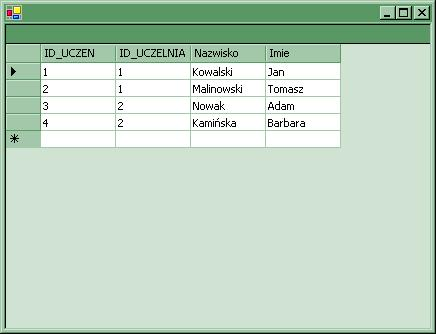
\includegraphics[width=0.50\textwidth]{./pic/swf07}
\caption{DataGrid związany z DataSet}
\end{center}
\end{figure}

\begin{scriptsize}
\begin{verbatim}
using System;
using System.Data;
using System.Data.SqlClient;
using System.Windows.Forms;

public class CMain : Form
{
  DataGrid dataGrid;

  public static string BuildConnectionString(string serverName, 
                                             string dbName, 
                                             string userName, 
                                             string passWd)
  {
    return String.Format(  
      @"Server={0};Database={1};User ID={2};Pwd={3};Connect Timeout=15", 
        serverName, dbName, userName, passWd);
  }

  public CMain()
  {
    // inicjuj DataGrid
    dataGrid = new DataGrid();
    dataGrid.Dock = DockStyle.Fill;
    this.Controls.Add( dataGrid );

    try
    {
      SqlConnection sqlConn = new SqlConnection();
      	
      sqlConn.ConnectionString = 
        BuildConnectionString( "(local)", "sqlTEST", "sa", String.Empty );

      sqlConn.Open();

      // inicjuj DataSet przy pomocy SqlDataAdapter
      SqlDataAdapter adapter = new SqlDataAdapter( 
        "SELECT * FROM T_STUDENT", sqlConn );
      // automatycznie twórz polecenia do wstawiania, modyfikacji i usuwania danych
      new SqlCommandBuilder( adapter );

      DataSet dataSet = new DataSet( "Dane" );
      // napełnij DataSet przez IDataAdapter
      adapter.Fill( dataSet );

      // powiąż DataGrid i DataSet 
      dataGrid.SetDataBinding( dataSet, "Table" );
      
      // zamknij połączenie
      sqlConn.Close();
    }
    catch ( Exception ex )
    {
      Console.WriteLine( ex.Message );
    } 
  }

  public static void Main()
  {
    Application.Run( new CMain() );
  }  
}
\end{verbatim}
\end{scriptsize}

Możliwości komponentu {\bf DataGrid} są naprawdę duże i szczegółowy ich opis zdecydowanie wykracza 
poza ramy tego skryptu. DataGrid może m.in. formatować komórki w zależności od ich zawartości czy
poprawnie obsługiwać relacje między danymi z wielu tabel. W przypadku aktualizacji danych w jednej z tabel,
DataGrid może reagować na to automatycznie odświeżając swoją zawartość.